\documentclass{article}
\usepackage[utf8]{inputenc}
\usepackage{pgfplots}
\usepackage[utf8]{inputenc}
\usepackage[shortlabels]{enumitem}
\usepackage{amsmath}
\usepackage{amssymb}
\usepackage{gensymb}
\usepackage{geometry}
\usepackage{listings}
\usepackage{xcolor}
\usepackage{pgfplots}
\usepackage{pgfplotstable}
\usepgfplotslibrary{fillbetween}
\pgfplotsset{compat=1.7}
\usepackage{tikz}
\geometry{
 a4paper,
 total={170mm,257mm},
 left=20mm,
 top=20mm,
}
\title{The Normal Distribution Unit}
\author{Andy Yan}
\date{January 2023}

\begin{document}

\maketitle

\section{Introduction}
\large{\textbf{PDF (Probability Density Function)}}\\
The probability per unit change of the variable at a particular point.\\
Instead of the dependent variable being probability \(P(X)\) it's replaced with \(pdf(X)\).\\

\begin{center}
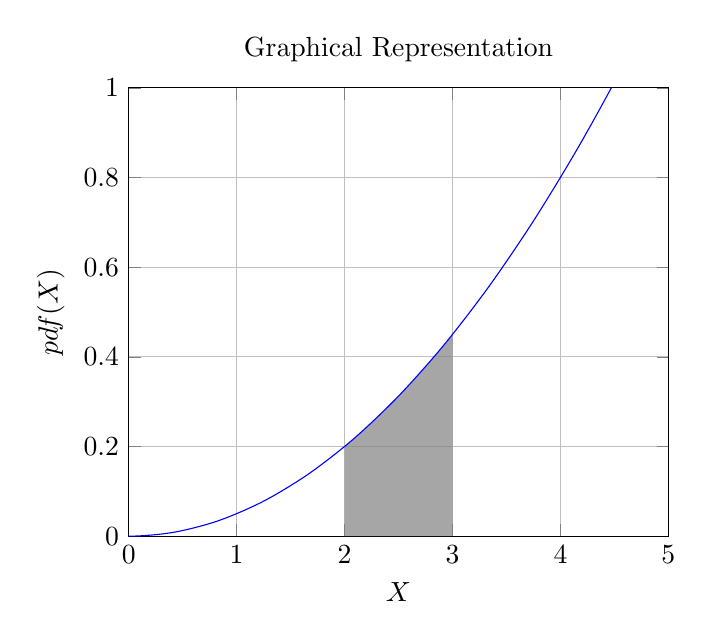
\begin{tikzpicture}
  \begin{axis}[
    xlabel=\(X\),
    ylabel=\(pdf(X)\),
    title = Graphical Representation,
    ymin = 0,
    ymax = 1,
    xmax = 5,
    xmin = 0,
    grid=major,
    no marks,
    ]
    \addplot+[smooth,blue,name path=A] {0.05*x*x}; % actual curve
    \addplot+[draw=none,name path=B] {0};     % “fictional” curve
    \addplot+[gray,opacity=0.7] fill between[of=A and B,soft clip={domain=2:3}]; % filling
  \end{axis}
\end{tikzpicture}
\end{center}
The shaded area represents \(P(2 < X < 3)\). NOTE: \(\leq\) and \(<\) are the same\\\\
\large{\textbf{Terms}}\\
Unitary Condition: Total Probability = 1\\
Continuous Random Variable: No breaks in continuity (All values exist within its range)\\
Unimodal: One mode/median/mean on the curve\\
Bimodal: Two modes/medians/means on the curve\\





\begin{minipage}[t]{0.5\textwidth}
\begin{center}
    Negatively Skewed / Skewed Left
    
\end{center}
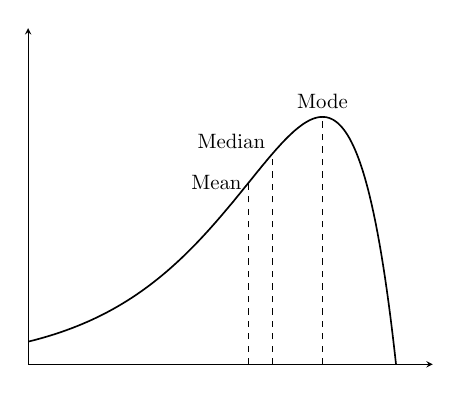
\begin{tikzpicture}[scale=0.75]
\begin{axis}[axis lines=left, ticks=none,xmax=0.5,ymax=0.5]
\addplot[thick,black, no markers, samples=200, domain=-5:0] {-x*exp(x)};
\draw[dashed] (axis cs:-1.68,0) -- (axis cs:-1.68,0.31) node [above, anchor=south east] {Median};
\draw[dashed] (axis cs:-2,0) -- (axis cs:-2,0.27) node [above, anchor=east] {Mean};
\draw[dashed] (axis cs:-1,0) -- (axis cs:-1,0.37) node [above] {Mode};
\end{axis}
\end{tikzpicture}
\end{minipage}
\begin{minipage}[t]{0.5\textwidth}
\begin{center}
    Positively Skewed / Skew Right 
\end{center}
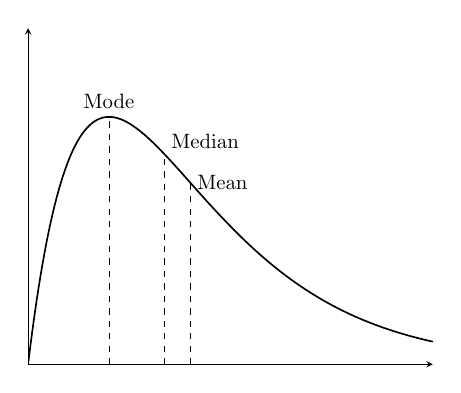
\begin{tikzpicture}[scale=0.75]
\begin{axis}[axis lines=left, ticks=none,xmin=0,ymax=0.5]
\addplot[thick,black, no markers, samples=200, domain=0:5] {abs(x)*exp(-x)};
\draw[dashed] (axis cs:1.68,0) -- (axis cs:1.68,0.31) node [above, anchor=south west] {Median};
\draw[dashed] (axis cs:2,0) -- (axis cs:2,0.27) node [above, anchor=west] {Mean};
\draw[dashed] (axis cs:1,0) -- (axis cs:1,0.37) node [above] {Mode};
\end{axis}
\end{tikzpicture}
\end{minipage}\\

\large{\textbf{Uniform Distribution}}\\
Probability Density remains constant.\\
\begin{center}
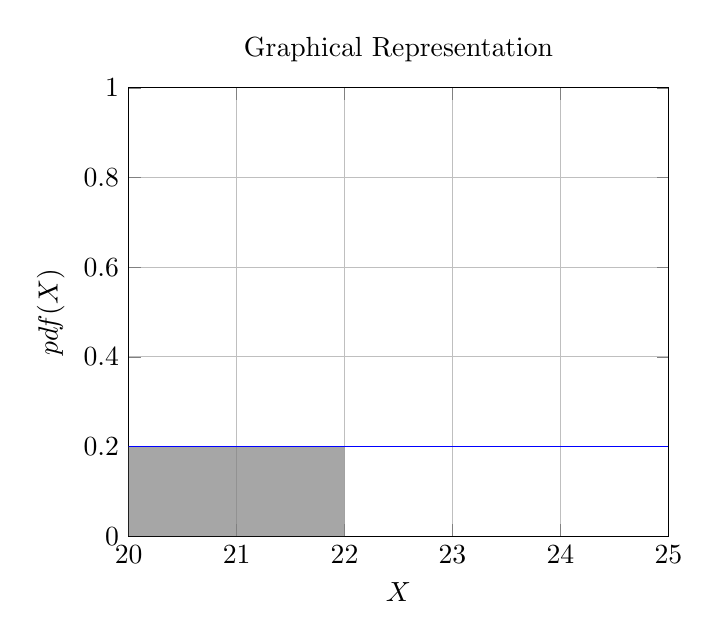
\begin{tikzpicture}
  \begin{axis}[
    xlabel=\(X\),
    ylabel=\(pdf(X)\),
    title = Graphical Representation,
    ymin = 0,
    ymax = 1,
    xmax = 25,
    xmin = 20,
    grid=major,
    no marks,
    ]
    \addplot+[smooth,blue,name path=A,domain = 0:25] {0.2}; % actual curve
    \addplot+[draw=none,name path=B,domain = 0:25] {0};     % “fictional” curve
    \addplot+[gray,opacity=0.7] fill between[of=A and B,soft clip={domain=20:22}]; % filling
  \end{axis}
\end{tikzpicture}
\end{center}\\
In this example, we are given \(a = \frac{1}{5}\).
\[P(20 < X < 22) = 2 \cdot a = 2 \cdot \frac{1}{5} = \frac{2}{5}\]
\large{\textbf{Probability Density}}\\
\[P(X < a) = ke^{-ka}\]
\(\mu\) : average time\\
\(k = \frac{1}{\mu}\) : \(\#\) of events per unit of time, ex. \(\#\)per hr/min/sec
\[\]
\large{\textbf{Exponential Distribution}}\\
Used to describe or find the probability related to time taken between 2 consecutive events that occurred.\\
\begin{center}
    \(P(X < x) = 1 - e^{-kx}\) WHITE\\
\(P(X > x) = e^{-kx}\) BLACK\\
\end{center}

\begin{center}
\begin{tikzpicture}[scale=0.8]
  \begin{axis}[
    xlabel=\(X\),
    ylabel=\(pdf(X)\),
    ymin = 0,
    ymax = 1,
    xmax = 5,
    xmin = 0,
    grid=major,
    no marks,
    ]
    \addplot+[smooth,blue,name path=A] {exp(-x)}; % actual curve
    \addplot+[draw=none,name path=B] {0};     % “fictional” curve
    \addplot+[white] fill between[of=A and B,soft clip={domain=0:2}]; % filling
    \addplot+[black] fill between[of=A and B,soft clip={domain=2:5}];
  \end{axis}
\end{tikzpicture}
\end{center}
Example: if \(x = 8, \mu = 10mins\)
\[P(X < 8) = 1 - e^{-\frac{1}{10}\cdot8} \approx 0.55mins\]

\section{Normal Distribution}
\begin{center}
    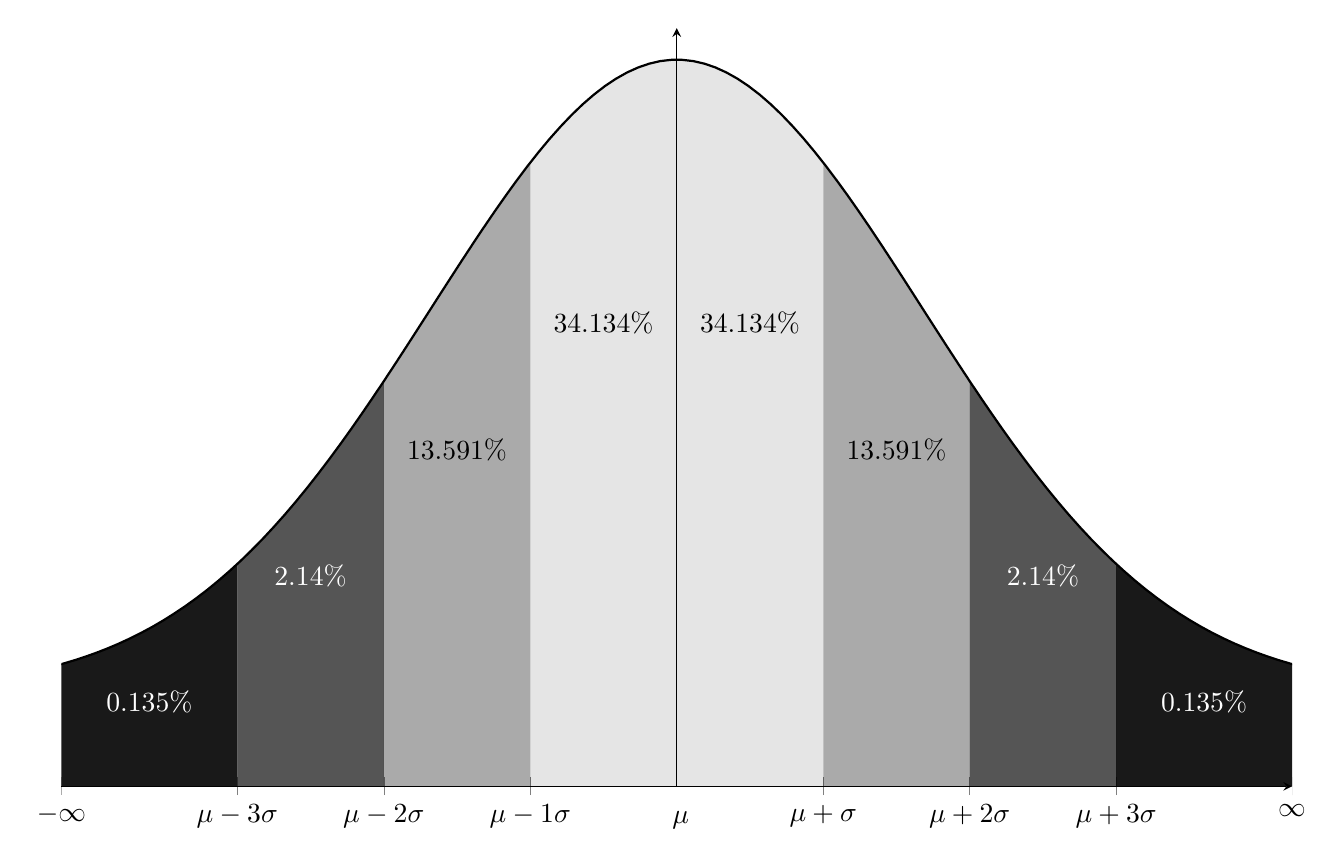
\begin{tikzpicture}[scale=1.5]
\begin{axis}[axis lines=middle,
            x label style={at={(axis description cs:0.2045,-0.0135)},anchor=north},
            xlabel = \(\mu\),
            width=12cm,
            height=8cm,
            ytick=\empty,
            xmax=2.8,
            xmin=-2.8,
            ymax=1.2,
            xtick={-2.8,-2,-4/3,-2/3,0,2/3,4/3,2,2.8},
            xticklabels={\(-\infty\),\(\mu-3\sigma\),\(\mu-2\sigma\),\(\mu-1\sigma\),\(\mu\),\(\mu+\sigma\),\(\mu+2\sigma\),\(\mu+3\sigma\),\(\infty\)},
            ]
\addplot[thick,black, no markers,samples=200,name path=A] {exp(-0.4*x^2)+0.15};
\addplot+[draw=none,no markers,name path=B] {0};
\addplot+[black,opacity=0.9] fill between[of=A and B,soft clip={domain=-5:-2}];
\addplot+[black,opacity=0.6666666] fill between[of=A and B,soft clip={domain=-2:-4/3}];
\addplot+[black,opacity=0.3333333] fill between[of=A and B,soft clip={domain=-1.33333333:-0.6666666666666666666666666666666666}];
\addplot+[black,opacity=0.1] fill between[of=A and B,soft clip={domain=-0.66666666666666666666666666666666666666666:0}];
\addplot+[black,opacity=0.9] fill between[of=A and B,soft clip={domain=2:5}];
\addplot+[black,opacity=0.666666666] fill between[of=A and B,soft clip={domain=1.333333333333333333333333333333333333:2}];
\addplot+[black,opacity=0.333333333] fill between[of=A and B,soft clip={domain=0.6666666666666666666666666666666666:1.333333333333333333333333333333333333}];
\addplot+[black,opacity=0.1] fill between[of=A and B,soft clip={domain=0:0.66666666666666666666666666666666666666666}];
\draw[draw=none] (axis cs:-1,0) -- (axis cs:-1,0.5) node [above] {\(13.591\%\)};
\draw[draw=none,text=white] (axis cs:-1,0) -- (axis cs:-5/3,0.3) node [above] {\(2.14\%\)};
\draw[draw=none,text=white] (axis cs:-1,0) -- (axis cs:-12/5,0.1) node [above] {\(0.135\%\)};
\draw[draw=none,] (axis cs:-1,0) -- (axis cs:-1/3,0.7) node [above] {\(34.134\%\)};
\draw[draw=none,] (axis cs:-1,0) -- (axis cs:1/3,0.7) node [above] {\(34.134\%\)};
\draw[draw=none] (axis cs:-1,0) -- (axis cs:1,0.5) node [above] {\(13.591\%\)};
\draw[draw=none,text=white] (axis cs:-1,0) -- (axis cs:5/3,0.3) node [above] {\(2.14\%\)};
\draw[draw=none,text=white] (axis cs:-1,0) -- (axis cs:12/5,0.1) node [above] {\(0.135\%\)};

\end{axis}
\end{tikzpicture}
\end{center}\
\large{\textbf{Properties of Normal Distribution}}\\
General Properties: Bell Shape, Symmetric, origin represents \(\mu\), total area under curve = 1\\
Distribution Type: Continuous Probability Distribution\\
y-axis represents pdf \& area under curve represents probability\\

\begin{minipage}[t]{0.5\textwidth}
\begin{center}
    Formula:
\end{center}
    \Large \[pdf(x) = \frac{1}{\sigma\sqrt{2\pi}}e^{\frac{1}{2}(\frac{x-\mu}{\sigma})^2}\]
\end{minipage}
\begin{minipage}[t]{0.5\textwidth}
\begin{center}
    \(x\) : random variable\\
    \(\mu\) : mean\\
    \(\sigma\) : Standard Deviation
\end{center}
\end{minipage}
\[\]
Exponent \((\frac{x-\mu}{\sigma})^2\) Properties:\\
When \(x = \mu\), \(f(x)\) has the maximum value. The greater \(|x - \mu|\) is, the less \(f(x)\) is.\\

\large \textbf{Probability for Standard Normal Distribution}\\
Each area interval of \(\mu \pm \textit{Z}\sigma\) (\textit{Z} = \(\{0,\pm1,\pm2,\pm3\}\)) represents a constant percentage which is the probability.
\[P(a \leq x \leq b) = \textbf{Sum of area intervals a to b} = \int_{a}^{b} \frac{e^{\frac{1}{2}(\frac{x-\mu}{\sigma})^2}}{\sigma\sqrt{2\pi}} \,dx \textit{  only to check answer}\]
\large \textbf{Using \textit{Z}-score} \(\textit{Z} = \frac{x-\mu}{\sigma}\)\\
If \textit{Z}-score isn't whole: \(x = \mu + \textit{Z}(\sigma)\)\\
Using \textit{Z}-score table to find \textit{Z}. Using positive table for positive \textit{Z}-score and vice versa. Row represents hundredth digits, add the row and the column to find desired \textit{Z}-score.
\[P(X<x) = P(\textit{Z} < \frac{x-\mu}{\sigma})\]
\[P(\textit{Z} < -x) = 1 - P(\textit{Z} < x)\]

\section{Normal Sampling and Modelling}
\large \textbf{Normal Sampling}
\begin{enumerate}
    \item The distribution of frequencies in the sample data tends to follow the bell-shaped curve as the underlying distribution.
    \item The sample mean (\(\bar{x}\)) estimates the population mean (\(\mu\))
    \item The sample standard deviation (\(s\)) estimates the population standard deviation (\(\sigma\))
    \item The larger the sample of a normal population, the more reliable the data will be in reflecting the underlying population
\end{enumerate}
\[\bar{x} = \frac{\sum x}{n}\]
\[s = \sqrt{\frac{\sum x^2 - n(\bar{x})^2}{n-1}}\]
\begin{center}
    \begin{tikzpicture}[scale=1]
\begin{axis}[axis lines=middle,
            ticks=none,
            width=12cm,
            height=8cm,
            x label style={at={(axis description cs:0.5,0)},anchor=north},
            xlabel = \(\mu \approx \bar{x}\),
            xmax=2.8,
            xmin=-2.8,
            ymax=1.2,
            ]
    \addplot[thick,black, no markers,samples=200,name path=A] {exp(-0.4*x^2)+0.15};
    \draw[dashed] (axis cs:1,0) -- (axis cs:1,0.82) node [] {};
    \draw[draw=none] (axis cs:1,0) -- (axis cs:0.5,0.3) node [] {\(\sigma \approx s\)};
    \draw[draw=none] (axis cs:1,0) -- (axis cs:0.5,0.25) node [] {\(\leftarrow\rightarrow\)};
\end{axis}
\end{tikzpicture}
\end{center}
\large \textbf{Normal Modelling}\\
Being sensible: \(\mu \pm \textit{Z}\sigma\) shouldn't create any unreasonable data such as negative time, beyond capacity, etc.\\
Discrete data can sometimes be modelled by a normal distribution. The standard normal curve can be used to approximate the area under the curve which can be used to solve problems involving probability.\\
\[\]
\large \textbf{Continuity Correction}\\
A continuity correction factor is used when you use a continuous probability distribution to approximate a discrete probability distribution.
\begin{itemize}
    \item \textbf{\(P(X \leq a)\)} \(\approx\) \(P(X < a  + 0.5)\)
    \item \textbf{\(P(X < a)\)} \(\approx\) \(P(X < a - 0.5)\)
    \item \textbf{\(P(X \geq a)\)} \(\approx\) \(P(X > a - 0.5)\)
    \item \textbf{\(P(X > a)\)} \(\approx\) \(P(X > a + 0.5)\)
    \item \textbf{\(P(X = a)\)} \(\approx\) \(P(a - 0.5 < X < a + 0.5)\)
\end{itemize}
Example:
\[P(X = 25) \rightarrow P(24.5 < X < 25.5)\]

\section{Normal Approximation}
REMEMBER the binomial distribution is perfectly symmetric if \(p = \frac{1}{2}\), and has some skewness when not. The normal approximation works bets when \(p\) is close to \(\frac{1}{2}\), and when \(n\) is large.
\[P(X \leq x) = \displaystyle\sum\limits_{k=0}^{x}\binom{n}{k}p^kq^{n-k} \]
The normal approximation is reasonable if both \(np \geq 5\) and \(n(1 - p) \geq 5\).\\\\
Fora binomial random variable \(X\):
\[\mu = np\]
\[\sigma^2 = np(1 - p) = npq\]
\large \textbf{Continuity Correction}
\begin{center}
    \def\arraystretch{1.5}
    {\setlength{\tabcolsep}{3em}
    \begin{tabular}{ c|c }
    Desired Probability & Normal Approximation\\
    \hline
    \(P(X \geq x)\) & \(P(\textit{Z} > \frac{(x-0.5)-\mu}{\sigma})\)\\
    \(P(X > x)\) & \(P(\textit{Z} > \frac{(x+0.5)-\mu}{\sigma})\)\\
    \(P(X \leq x)\) & \(P(\textit{Z} < \frac{(x+0.5)-\mu}{\sigma})\)\\
    \(P(X < x)\) & \(P(\textit{Z} < \frac{(x-0.5)-\mu}{\sigma})\)\\
    \end{tabular}
\end{center}
\section{Repeated Sampling and Hypothesis Testing}\
\large \textbf{Repeated Sampling}\\
When repeated samples of the same size are drawn from a normal population, the sample means will be normally distributed with a mean equal to the population mean (\(\mu_{\Bar{x}} = \mu\)). The distribution of sample means will be where \(n\) is the sample size:
\[\sigma_{\Bar{x}} = \frac{\sigma}{\sqrt{n}}\]
To find a \textit{Z}-score for a sample mean:
\[P(\Bar{x} < x) =  P(\textit{Z} < \frac{(x-0.5)-\mu_{\Bar{X}}}{\sigma_{\Bar{x}}})\]
\large \textbf{Hypothesis Testing}\\
A hypothesis test consists of a null hypothesis \(H_0\) and an alternative hypothesis \(H_1\). The null hypothesis is being challenged is for example \(H_0\): \(\mu = 45\). While we suspect \(H_1\) :\(\mu < 45\). To obtain a sample mean \(\mu_{\Bar{x}} = 44.5\) is very rare, and getting such will prove \(\mu \neq 45\).
Our next step is to establish a decision rule. The significance level \(\alpha\) is the probability threshold for us to determine if observed results are rare enough to justifying rejecting \(H_0\). For example, if \(\alpha = 0.05\), we are willing to be wrong 5\% of the time. We are given \(\sigma = 2, n = 30\). To begin the test, we assume \(H_0\) is true:

\[P(\Bar{x} < \mu_{\Bar{x}}) =  P(\textit{Z} < \frac{\mu_{\Bar{x}}-\mu}{\sigma_{\Bar{x}}})\]
\[P(\Bar{x} < 44.5) =  P(\textit{Z} > \frac{44.5-45}{0.365}) = P(Z < -1.37) = 0.0835\]
To conclude, we compare our answer with \(\alpha\). If the probability is greater than the significance level we accept \(H_0\), else we accept \(H_1\). In this case \(0.0835 > \alpha\), therefore, the evidence isn't sufficient to refute our claim.




\end{document}
